\section{Methodology and tools}
Organizing the work is a crucial task in all projects, and for this reason the following sections contain not only a description of the methodology used to develop the tool, but also how other important elements in the development, like the version control or the testing and validation, were carried out.

\subsection{Waterfall model and monitoring tools}
\label{ssec:methodology}
To accomplish all of this tool's goals, it was important to use a methodology that fits its needs. The developed tool is composed of a series of scripts divided into different parts, which needed to be well defined in the design phase so the code could be developed in a simple, agile, and clean way.

Consequently, the waterfall methodology was used, which traditionally consists of a series of phases where each one must be completed before the next phase can begin, and there is no overlapping of them, as can be seen in figure \ref{img:waterfallModel}. 

\begin{figure}[!ht]
	\hspace{-1.5cm}
	\centering
	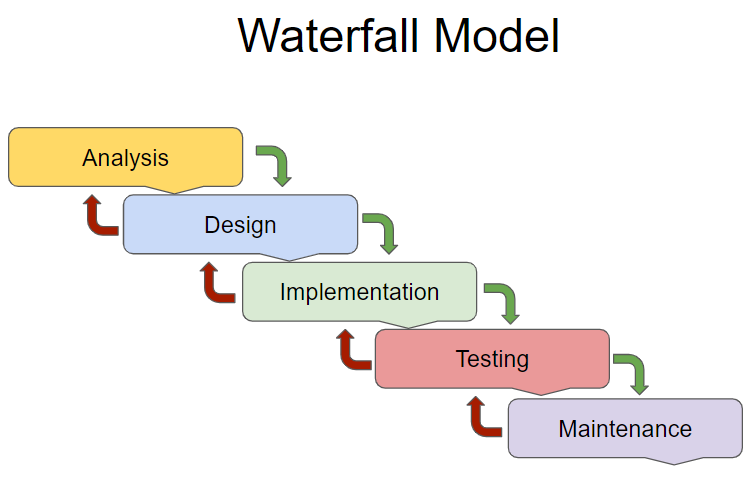
\includegraphics[width=10cm]{img/waterfall-model}
%	\caption{Example of the waterfall methodology, obtained from "learnlearn.uk".}
	\caption{Example of the waterfall methodology}
	\label{img:waterfallModel}
\end{figure}


However, in this case, some phases, like the design and the implementation, went through some iterations because some functions could not be developed the way they were designed. The implementation and testing iterated as well, as there were very distinct functionalities to develop and it was important to test them separately. 
More information about how this methodology has been implemented can be found in the subsection \ref{ssec:tasks} - \textit{Task description}.

\pagebreak
In addition, using a version control manager tool, like \texttt{git}, has been a key aspect, as it allows to undo recent changes (in the code, the design, the documentation, etc.) if an error is found some days after doing it, or to easily backup the project if the computer gets broken. 

Github\cite{ThisProjectGit} has also been used as a platform to upload all the files related to this project, since the developed tool is Open Source and it is usually better to use a repository hosting open to the Internet, to allow other people to test it and use it. 

All other tools used to build this project are explained in section \ref{ssec:resources} of this document.

\subsection{Testing and validation}
To consider a tool finished, it is necessary to have a validation process to be sure the automation works as intended. During the development, there have been several testing phases using virtual machines connected to the Internet, and tools like the \textit{Event Viewer} (Windows) or \texttt{watch} (Linux) have been used to spot changes easily in the operating system.

But a proper validation using different machines, networks, and configurations has not been achieved because of the lack of time, experience, and infrastructure. That is why it has been listed in the "future work" part of the conclusions (section \ref{ssec:futureWork}), as it could help to better adapt the tool to real-world environments.